\subsection{Definição do BOUNDED CONTEXT: DBFFileDefinition}
O DBFFileDefinition é o núcleo responsável por estabelecer a estrutura inicial de um arquivo .DBF. Ele assegura que a estrutura base seja válida e compatível com as regras do formato .DBF. Esse contexto gerencia a criação da "casca" do arquivo, preparando-o para operações futuras, como inserção de registros (DBFRecord) ou exportação (DBFExport).
Os arquivos .DBF seguem um formato binário rígido, onde cada componente: \\
 - DBFHeader (cabeçalho) \\
 - DBFField (campos) \\
 - DBFRecord (registros) \\
precisa estar corretamente alinhado e estruturado para garantir compatibilidade com sistemas que processam esse tipo de dado. Um erro na definição estrutural pode tornar o arquivo ilegível para outros sistemas, tornando a configuração correta da estrutura um aspecto crítico.
Esse contexto atua diretamente na criação da estrutura inicial de um .DBF. Ele define regras para nomes de campos, tipos de dados, tamanho dos registros e alinhamento da memória, garantindo que a estrutura seja construída corretamente desde o início. É importante ressaltar que, nesse estágio, as listas de campos (List<DBFField>) e registros (List<DBFRecord>) são inicializadas vazias. \\

\begin{bclogo}[logo=\bcattention, couleurBarre=red, noborder=true, 
    couleur=LightSalmon]{Important!}
    \begin{itemize}
        \item O DBFFileDefinition é responsável pela criação da "casca" inicial do arquivo .DBF.
        \item Neste contexto, as listas de campos (List<DBFField>) \\ e registros (List<DBFRecord>) são inicializadas vazias.
        \item A validação completa do arquivo .DBF só deve ocorrer após a adição de dados e é responsabilidade de outro contexto (DBFValidation).
    \end{itemize}
\end{bclogo}

O DBFFileDefinition será modelado como um agregado (Aggregate Root), onde o DBFFile atuará como a raiz do agregado. Esse agregado encapsula toda a estrutura inicial do .DBF.
O DBFFile conterá as seguintes estruturas: 
\begin{itemize}
    \item DBFHeader: Metadados do .DBF, incluindo versão, data de modificação, contagem de registros e deslocamento do primeiro registro. \\
    \item List<DBFField>: Lista de campos (DBFField) que definem a estrutura do .DBF, incluindo nome, tipo de dado e tamanho. 
    \item List<DBFRecord>: Lista de registros (DBFRecord), que é inicializada vazia. 
\end{itemize}

\textbf{Esse agregado garantirá que:}
\begin{itemize}
    \item A estrutura inicial do .DBF seja consistente e válida.
    \item O DBFFileDefinition não gerencia a adição, remoção ou alteração de campos, nem a manipulação de registros. Essas são responsabilidades de outros Bounded Contexts.
\end{itemize}

\subsection{Organização do DBFFileDefinition}

O DBFFileDefinition é responsável pela criação da estrutura inicial do .DBF, garantindo que ele seja construído de maneira válida e coerente. Ele tem como foco exclusivo a definição da "casca" do arquivo, ou seja, a estrutura base, preparando-o para receber dados e ser utilizado por outros contextos. Este contexto não gerencia a modificação de campos (DBFField) ou a manipulação de registros (DBFRecord).\\

\textbf{Responsabilidades Exclusivas:} 

\begin{enumerate}
    \item O DBFFileDefinition não gerencia a adição, remoção ou alteração de campos (DBFField).
    \item O DBFFileDefinition não gerencia a manipulação de registros (DBFRecord).
    \item Essas responsabilidades são delegadas aos Bounded Contexts DBFFieldManagement e DBFRecordManagement, respectivamente.
\end{enumerate}

\subsection{Como Esse Contexto Será Implementado?}
O DBFFileDefinition será modelado como um agregado (Aggregate Root), onde o DBFFile atuará como a raiz do agregado. Esse agregado encapsula a estrutura inicial do .DBF, representando a "casca" do arquivo.
\subsubsection{Tarefas Principais do DBFFileDefinition}
O DBFFileDefinition tem como tarefas principais a criação da estrutura inicial do .DBF e a preparação para sua utilização por outros contextos. \\\\
\textbf{Gerenciamento da Estrutura Inicial:} \\\\
- Criar um novo arquivo .DBF, definindo o cabeçalho (DBFHeader) e inicializando a lista de campos (List<DBFField>) e a lista de registros (List<DBFRecord>) como vazias. \\
- Garantir que o tamanho do cabeçalho seja calculado corretamente. \\
- Determinar a posição (offset) do primeiro registro dentro do arquivo. \\\\
\textbf{Preparação para Outros Contextos:} \\\\
- Fornecer a "casca" do .DBF pronta para ser populada com dados e validada (DBFValidation). \\
- Garantir que a estrutura inicial definida seja compatível com a exportação (DBFExport). \\

\subsubsection{Tipos de dados do DBFFileDefinition}
\textbf{Esta seção detalha os tipos de dados utilizados no contexto DBFFileDefinition, suas propriedades e as regras de negócio associadas}

\subsubsection{Informações gerais do DBFFile}
\begin{itemize}
    \item \textbf{Nome do dado}: \textit{\textbf{DBFFile}}
    \item \textbf{Tipo do dado}: \textit{\textbf{Aggregate Root}}
    \item \textbf{Descrição do dado}: O \textit{\textbf{DBFFile}} é a raiz do agregado e centraliza todas as regras de criação e manipulação da estrutura do \textit{\textbf{.dbf}}. Ele encapsula o cabeçalho: \textit{\textbf{DBFHeader}}, a lista de campos:\textit{\textbf{List<DBFField>}} e os registros:\textit{\textbf{List<DBFRecord>}}, garantindo que nenhuma modificação ocorra de maneira inconsistente.
\end{itemize}


\begin{table}[H]
    \centering
    \textbf{Atributos do Aggregate Root DBFFile}
    \begin{tabular}{|p{0.2\textwidth} | p{0.3\textwidth} | p{0.5\textwidth}|}
        \hline
        \textbf{Atributo} & \textbf{Tipo} & \textbf{Descrição} \\
        \hline
        name & string & Nome do arquivo .DBF. \\
        \hline
        header & DBFHeader & Metadados do .DBF (versão, data, quantidade de registros). \\
        \hline
        fields & List<DBFField> & Lista de colunas (campos da tabela). \\
        \hline
        records & List<DBFRecord> & Lista de registros armazenados dentro do .DBF. \\
        \hline
        recordSize & number & Define o tamanho dos Registros deste dbf, sendo calculado pela soma em bytes dos CAMPOS do arquivo \\
        \hline
    \end{tabular}
    \caption{Atributos do DBFFile e suas descrições}
    \label{tab:tabela_atributos_dbffile}
\end{table}

\subsubsection{Metodos que estão dentro do DBFFile}
\begin{itemize}
    \item \textbf{create}: Método responsável por criar a instancia do DBFFile, A implementação não amarra como será feita, caso queira usar um factory ou um builder, a seu criterio. Sempre uma nova instancia for criada, lembre-se que os campos fields e records devem ser listas vazias. O DBFHeader não pode está vazia.
    \item \textbf{calculateRecordSize}: Método responsável por calcular o tamanho da soma de todos os campos: \textit{\textbf{DBFField}} em bytes.
    \item \textbf{validateHeaderSize}: Método responsável por validar o tamanho do cabeçalho, o tamanho do cabeçalho deve ser múltiplo de 32 bytes. Ou seja, caso o tamanho do cabeçalho em bytes for um numero que não é multiplo de 32, o sistema tem que adicionar a quantidade de bytes com zeros até que o tamanho seja múltiplo de 32.
\end{itemize}

\subsubsection{Informações Gerais do DBFField}
\textbf{Nome do dado}: \textit{\textbf{DBFField}} \\  
\textbf{Tipo do dado}: Entidade \\  
\textbf{Descrição do dado}: Cada DBFField representa um campo dentro do \textit{\textbf{.bdf}}, definindo nome, tipo, tamanho e alinhamento dos dados armazenados. \\  

\begin{table}[H]
    \centering
    \textbf{Atributos da entidade do DBFField}
    \begin{tabular}{|p{0.2\textwidth} | p{0.3\textwidth} | p{0.5\textwidth}|}
        \hline
        \textbf{Atributo} & \textbf{Tipo} & \textbf{Descrição} \\
        \hline
        name & string & Nome do campo da tabela \\
        \hline
        type & enum &  Um enumerador com os valores permitidos: ver os valores na tabela do enum abaixo. \\
        \hline
        size & number  & Tamanho do campo em bytes. \\
        \hline
        decimal & number  & Aqui fica qual o número de casas decimais que será colocado, quando os registros forem escritos. Exemplo: Caso você queira o numero 12 e coloque no tamanho do campo sendo 2, está tudo bem, pois o binario será: 0x31 0x32. Porém se for colocado no tamanho do campo 5 bytes e só dois decimais, ai a representação do numero será: 0x31 0x32 0x2E 0x30 0x30, Pois obrigatoriamente quando é colocado só 2 decimais o resto será flutuante, então será 1 caracter para o ponto e outros dois para zeros \\
        \hline
    \end{tabular}
    \caption{Atributos do DBFField e suas descrições}
    \label{tab:tabela_atributos_dbffield}
\end{table}

\begin{table}[H]
    \centering
    \textbf{Enumerator do campo type do DBFField}
    \begin{tabular}{|p{0.2\textwidth} | p{0.3\textwidth} | p{0.5\textwidth}|}
        \hline
        \textbf{Atributo} & \textbf{Tipo} & \textbf{Descrição} \\
        \hline
        C & Character & É um tipo que aceita textos, porém com o tamanho máximo sendo de 10 bytes \\
        \hline
        N & Numeric &  É um tipo que aceita numeros em geral, tanto decimais, quanto inteiros, porém com um tamanho máximo de 19 bytes \\
        \hline
        F & Float  & É um tipo que aceita as mesmas regras do Numeric, porém é para numeros flutuantes com menor precisão \\
        \hline
        L & Logical  & Booleano (T ou F, para verdadeiro ou falso). Sendo seu maximo 1 byte \\
        \hline
        D & Date  & Data no formato YYYYMMDD (8 caracteres). \\
        \hline
    \end{tabular}
    \caption{Todos os valores possiveis que podem ser escolhidos para o campo type do \textit{\textbf{DBFField}}}
    \label{tab:tabela_enumeracao_atributo_type}
\end{table}

\subsubsection{Metodos que estão dentro do DBFFile}
\begin{itemize}
    \item \textbf{create}: Método responsável por criar a instancia do \textit{\textbf{DBFField}}, Ou seja ele cria um BDFFiel válido para ser colocado dentro da lista de \textit{\textbf{DBFField}}.
    \item \textbf{validateNameField}: Método responsável por validar o nome do campo, o nome do campo não pode ser vazio, e nem pode ter mais de 10 caracteres. 
    \item \textbf{calculateSize}: Calcula o tamanho do campo em bytes, baseado no tipo de dado. Caso não contenha já registros, se sim pegue o maior registro deste campo e coloque como o tamanho.
    \item \textbf{validateDecimal}: Calcula se o valor de decimais é um numero inteiro válido, seguindo a formula: \\
    \subitem \( I = P - (D + 1) \)  
    \subitem Onde:  
    \begin{itemize}
        \item \( I \) é o número máximo de dígitos inteiros.  
        \item \( P \) é o tamanho total do campo (quantidade máxima de caracteres permitidos).  
        \item \( D \) é o número de casas decimais.  
    \end{itemize}
    
    \subitem \textbf{Exemplos práticos: } 
    \begin{itemize}
        \item Suponha que \( P = 6 \) e \( D = 2 \).  
        \item Aplicando a fórmula:  
        \[
        I = 6 - (2 + 1) = 3
        \]
        \item Isso significa que o número pode ter, no máximo, \textbf{3 dígitos inteiros}.  
    \end{itemize}
    
    \subitem \textbf{Explicação detalhada:}  
    \begin{itemize}
        \item O valor de \( P = 6 \) indica que o campo pode armazenar \textbf{até 6 bytes} no total.  
        \item Além disso, o próprio \textbf{ponto decimal (`.`) ocupa 1 byte}, representado em binário como \textit{\textbf{0x2E}}.  
        \item Isso deixa \textbf{3 bytes disponíveis} para os dígitos inteiros.  
        \item Como cada número inteiro ocupa \textbf{1 byte por caractere}, o maior número que pode ser armazenado é \textbf{999}.  
        \item O número \textbf{1000} não cabe, pois precisaria de \textbf{4 bytes para os dígitos inteiros}, excedendo o limite permitido.  
    \end{itemize}
\end{itemize}
\begin{figure}[H]
    \begin{equation}
        I \leq P - (D + 1), \quad {se } D > 0
        \end{equation}
        
        \begin{equation}
        I \leq P, \quad {se } D = 0
    \end{equation}
    \caption{Fórmula para cálculo do número máximo de dígitos inteiros}
\end{figure}


\subsubsection{Informações Gerais do DBFRecord}
\textbf{Nome do dado}: \textit{\textbf{DBFRecord}} \\  
\textbf{Tipo do dado}: Entidade \\  
\textbf{Descrição do dado}: Cada \textit{\textbf{DBFRecord}} representa uma linha de dados dentro do \textit{\textbf{.bdf}}, contendo valores para cada \textit{\textbf{DBFField}} definido. Os registros devem seguir estritamente o formato dos campos \textit{\textbf{DBFField}} definidos na estrutura do \textit{\textbf{.bdf}} \\  

\begin{table}[H]
    \centering
    \textbf{Atributos da entidade do DBFRecord}
    \begin{tabular}{|p{0.2\textwidth} | p{0.3\textwidth} | p{0.5\textwidth}|}
        \hline
        \textbf{Atributo} & \textbf{Tipo} & \textbf{Descrição} \\
        \hline
        value & Map<string,any> & Estrutura de chave/valor que armazena os dados de um registro, onde a chave é o nome do campo (DBFField.name) e o valor é o dado armazenado. \\
        \hline
        isDeleted & boolean & Indica se o registro foi logicamente marcado como excluído (0x2A). \\
        \hline
    \end{tabular}
    \caption{Atributos do DBFRecord e suas descrições}
    \label{tab:tabela_atributos_dbfrecord}
\end{table}
\textbf{TODO: ESCREVER SOBRE OS METODOS DO DBFRecord, ESCRITO EM 19/03/2025}
\subsubsection{Metodos que estão dentro do DBFRecord}
\begin{itemize}
    \item \textbf{create}: Método responsável por criar a instancia do DBFFile, A implementação não amarra como será feita, caso queira usar um factory ou um builder, a seu criterio. Sempre uma nova instancia for criada, lembre-se que os campos fields e records devem ser listas vazias. O DBFHeader não pode está vazia.
    \item \textbf{calculateRecordSize}: Método responsável por calcular o tamanho da soma de todos os campos: \textit{\textbf{DBFField}} em bytes.
    \item \textbf{validateHeaderSize}: Método responsável por validar o tamanho do cabeçalho, o tamanho do cabeçalho deve ser múltiplo de 32 bytes. Ou seja, caso o tamanho do cabeçalho em bytes for um numero que não é multiplo de 32, o sistema tem que adicionar a quantidade de bytes com zeros até que o tamanho seja múltiplo de 32.
\end{itemize}


\subsubsection{Informações Gerais do DBFHeader}
\textbf{Nome do dado}: \textit{\textbf{DBFHeader}} \\  
\textbf{Tipo do dado}: Entidade \\  
\textbf{Descrição do dado}: Cada DBFField representa um campo dentro do \textit{\textbf{.bdf}}, definindo nome, tipo, tamanho e alinhamento dos dados armazenados. \\  

\subsubsection{Atributos do DBFHeader}  
\textbf{version: enum} - Versão do `.DBF`. (`0x03` para `dBase III`). \\  
\textbf{lastUpdated: Date} - Data da última modificação do arquivo. \\  
\textbf{recordCount: number} - Número total de registros armazenados (`DBFRecord`). \\  
\textbf{firstRecordOffset: number} - Offset (posição em bytes) do primeiro registro dentro do arquivo. \\  

\subsubsection{Regras de negócio do DBFHeader}
\begin{enumerate}
    \item O offset do primeiro registro (`firstRecordOffset`) deve ser sempre múltiplo de 32 bytes.
    \item A versão do `.DBF` deve ser compatível (`0x03` para `dBase III`).
    \item O número de registros (`recordCount`) deve ser atualizado corretamente sempre que um registro (`DBFRecord`) for adicionado ou removido.
\end{enumerate}


\subsection{Diagrama de Classes do DBFFileDefinition}
\begin{figure}[H]
    \centering
    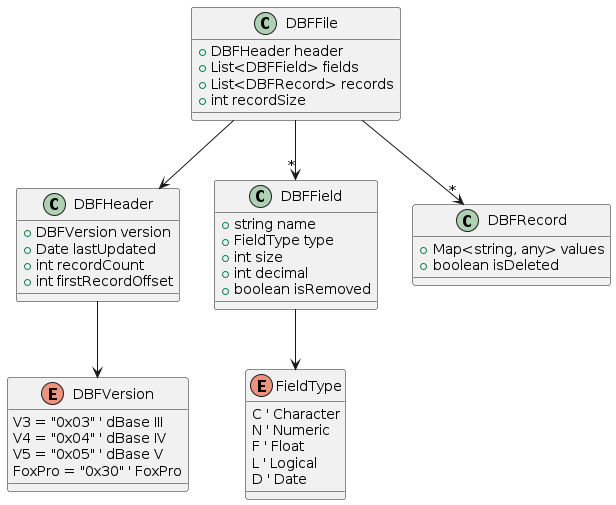
\includegraphics[width=1\textwidth]{image/uml_DBFESTRUCTURE.png}
    \caption{Diagrama de Classes do Bounded Context: DBFFileDefinition}
\end{figure}

\subsection{BDD do caso de uso: CreateDBFFileBaseV3}
\subsubsection{Feature: Criar um objeto DBFFile válido}
Como um usuário ou sistema \\
Quero criar um objeto \textbf{DBFFile} contendo: \\
- \textbf{DBFHeader}\\
- \textbf{List<DBFField>} \\
- \textbf{List<DBFRecord>}\\
inicializados corretamente Para que ele possa ser utilizado posteriormente por outros casos de uso \\

\subsubsection{Background}
\textbf{Given} que \textbf{DBFFile} representa um arquivo `.DBF` na memória \\
\textbf{And} \textbf{DBFFile} deve ser criado apenas com: \\
- \textbf{DBFHeader} \\
- \textbf{List<DBFField>}\\
- \textbf{List<DBFRecord>}\\
todos inicializados corretamente

\subsubsection{Scenario: Criar um objeto DBFFile com campos e registros válidos}
\textbf{Given} que o sistema inicia a criação de um \textbf{DBFFile} \\
\textbf{When} o sistema cria um \textbf{DBFHeader} \\
\textbf{And} o \textbf{DBFHeader} contém a versão padrão do `.DBF` (`0x03`) \\
\textbf{And} o \textbf{DBFHeader} contém a data atual como última modificação \\
\textbf{And} o \textbf{DBFHeader} tem o número total de registros inicializado como zero \\
\textbf{And} o \textbf{DBFHeader} calcula a posição inicial onde os registros serão armazenados \\
\textbf{And} o sistema inicializa uma \textbf{List<DBFField>} vazia \\
\textbf{And} o sistema inicializa uma \textbf{List<DBFRecord>} vazia \\
\textbf{Then} o sistema associa o \textbf{DBFHeader}, \textbf{List<DBFField>} e \textbf{List<DBFRecord>} ao \textbf{DBFFile} \\
\textbf{And} o sistema retorna um \textbf{DBFFile} pronto para ser manipulado \\

\subsubsection{Scenario: Criar um DBFFile sem registros iniciais}
\textbf{Given} que o sistema inicia a criação de um \textbf{DBFFile} \\
\textbf{When} o sistema cria um \textbf{DBFHeader} \\
\textbf{And} o sistema inicializa uma \textbf{List<DBFField>} vazia \\
\textbf{And} a \textbf{List<DBFRecord>} está vazia, pois não há registros no momento da criação \\
\textbf{Then} o sistema retorna um \textbf{DBFFile} válido contendo apenas cabeçalho e campos \\

\subsubsection{Scenario: Falha ao criar o DBFHeader}
\textbf{Given} que ocorreu um erro ao criar o \textbf{DBFHeader} \\
\textbf{When} o sistema tenta associar o \textbf{DBFHeader} ao \textbf{DBFFile} \\
\textbf{Then} o sistema deve lançar um erro \textbf{"Erro: Falha ao criar o cabeçalho do DBF"} \\
\textbf{And} o sistema não deve criar um \textbf{DBFFile} \\

\subsubsection{Scenario: Falha ao inicializar a lista de campos (`DBFField`)}
\textbf{Given} que ocorreu um erro ao criar a \textbf{List<DBFField>} vazia \\
\textbf{When} o sistema tenta associar a lista de campos ao \textbf{DBFFile} \\
\textbf{Then} o sistema deve lançar um erro \textbf{"Erro: A lista de campos deve ser inicializada vazia"} \\
\textbf{And} o sistema não deve criar um \textbf{DBFFile} \\

\subsubsection{Scenario: Falha ao inicializar a lista de registros (`DBFRecord`)}
\textbf{Given} que ocorreu um erro ao criar a \textbf{List<DBFRecord>} vazia \\
\textbf{When} o sistema tenta associar a lista de registros ao \textbf{DBFFile} \\
\textbf{Then} o sistema deve lançar um erro \textbf{"Erro: A lista de registros deve ser inicializada vazia"} \\
\textbf{And} o sistema não deve criar um \textbf{DBFFile} \\

\subsubsection{Scenario: Falha ao definir a versão do `.DBF`}
\textbf{Given} que o sistema inicia a criação de um \textbf{DBFFile} \\
\textbf{When} o sistema cria um \textbf{DBFHeader} \\
\textbf{And} a versão do `.DBF` não pode ser definida corretamente \\
\textbf{Then} o sistema deve lançar um erro \textbf{"Erro: Versão do `.DBF` inválida"} \\
\textbf{And} o sistema não deve criar um \textbf{DBFFile} \\

\subsubsection{Scenario: Falha ao definir a data da última modificação}
\textbf{Given} que o sistema inicia a criação de um \textbf{DBFFile} \\
\textbf{When} o sistema cria um \textbf{DBFHeader} \\
\textbf{And} ocorre um erro ao definir a data da última modificação \\
\textbf{Then} o sistema deve lançar um erro \textbf{"Erro: Data de modificação inválida"} \\
\textbf{And} o sistema não deve criar um \textbf{DBFFile} \\

\subsubsection{Scenario: Falha ao calcular o offset do primeiro registro}
\textbf{Given} que o sistema inicia a criação de um \textbf{DBFFile} \\
\textbf{When} o sistema cria um \textbf{DBFHeader} \\
\textbf{And} ocorre um erro ao calcular a posição inicial do primeiro registro \\
\textbf{Then} o sistema deve lançar um erro \textbf{"Erro: Falha ao calcular o offset do primeiro registro"} \\
\textbf{And} o sistema não deve criar um \textbf{DBFFile} \\

